%******************************************************** -*-LaTeX-*- ******************************
%                                                                                                  *
% v3.0.2.0.2 Relationen und Funktionen - Geometrisches Bild.tex                                    *
%                                                                                                  *
% Copyright (C) 2023 Kategory GmbH \& Co. KG (joerg.kunze@kategory.de)                             *
%                                                                                                  *
% v3.0.2.0.2 Relationen und Funktionen - Geometrisches Bild is part of kategoryMathematik.         *
%                                                                                                  *
% kategoryMathematik is free software: you can redistribute it and/or modify                       *
% it under the terms of the GNU General Public License as published by                             *
% the Free Software Foundation, either version 3 of the License, or                                *
% (at your option) any later version.                                                              *
%                                                                                                  *
% kategoryMathematik is distributed in the hope that it will be useful,                            *
% but WITHOUT ANY WARRANTY; without even the implied warranty of                                   *
% MERCHANTABILITY or FITNESS FOR A PARTICULAR PURPOSE.  See the                                    *
% GNU General Public License for more details.                                                     *
%                                                                                                  *
% You should have received a copy of the GNU General Public License                                *
% along with this program.  If not, see <http://www.gnu.org/licenses/>.                            *
%                                                                                                  *
%***************************************************************************************************

\documentclass[a4paper]{amsart}
% \documentclass[a4paper]{book}

%-----------------------------------------------------------------------------------------------------*
% package:                                                                                            *
%-----------------------------------------------------------------------------------------------------*
\usepackage{amssymb}
\usepackage{amsfonts}
\usepackage{amsmath}
\usepackage{amsthm}

\usepackage{mathabx}

\usepackage{a4wide} % a little bit smaller margins

\usepackage{graphicx}
\usepackage{hyperref}
\usepackage{algorithmic}
\usepackage{listings}
\usepackage{color}
\usepackage{colortbl}
\usepackage{sidecap}
\usepackage{comment}
\usepackage{tcolorbox}
\usepackage{collect}

\usepackage{upgreek}

% \usepackage{diagrams}

\usepackage[german]{babel}
\usepackage[none]{hyphenat}
\emergencystretch=4em

\usepackage[utf8]{inputenc} % to be able to use äöü as characters in text
\usepackage[T1]{fontenc} % to be able to use äöü in lables
\usepackage{lmodern}     % to avoid pixelation introduced by fontenc

\usepackage{hyperref}

\usepackage{tikz}
\usepackage{tikz-cd}
\usetikzlibrary{babel}

%-----------------------------------------------------------------------------------------------------*
% theorem:                                                                                            *
%-----------------------------------------------------------------------------------------------------*
\theoremstyle{definition}
\newtheorem{theorem}{Theorem}[subsection]

\newcommand{\myTheorem}[1]{%
  \newtheorem{jk#1}[theorem]{#1}
  \newenvironment{#1}[1]{%
    \expandafter\begin{jk#1} \expandafter\label{#1:##1}\textbf{(##1):}
  }{%
    \expandafter\end{jk#1}
  }
}

\myTheorem{Definition}
\myTheorem{Proposition}
\myTheorem{Theorem}
\myTheorem{Example}
\myTheorem{Remark}

\definecollection{jkjkFrage}
\newtheorem{jkFrage}[theorem]{Frage}
\newenvironment{Frage}[1]{%
  \expandafter\begin{jkFrage} \expandafter\label{Frage:#1}\textbf{(#1):}
  \begin{collect}{jkjkFrage}{}{}
    \item \ref{Frage:#1} #1
  \end{collect}
}{%
  \expandafter\end{jkFrage}
}

\newcommand{\myRef}[2]{[#1 \ref{#1:#2}, ``#2'']}

\renewcommand{\proofname}{Beweis}

%-----------------------------------------------------------------------------------------------------*
% operator:                                                                                           *
%-----------------------------------------------------------------------------------------------------*
\DeclareMathOperator{\End}{End}
\DeclareMathOperator{\Ker}{Ker}
\DeclareMathOperator{\Mat}{Mat}
\DeclareMathOperator{\rank}{rank}
\DeclareMathOperator{\ggT}{ggT}
\DeclareMathOperator{\len}{len}
\DeclareMathOperator{\ord}{ord}
\DeclareMathOperator{\kgV}{kgV}
\DeclareMathOperator{\id}{id}
\DeclareMathOperator{\red}{red}
\DeclareMathOperator{\supp}{supp}
\DeclareMathOperator{\Bild}{Bild}
\DeclareMathOperator{\Urbild}{Urbild}
\DeclareMathOperator{\Rang}{Rang}
\DeclareMathOperator{\Det}{Det}
\DeclareMathOperator{\Hom}{Hom}

\DeclareMathOperator{\sub}{sub}
\DeclareMathOperator{\blk}{blk}
\DeclareMathOperator{\minimal}{minimal}
\DeclareMathOperator{\maximal}{maximal}

\definecolor{mygreen}{rgb}{0,0.6,0}
\definecolor{mygray}{rgb}{0.5,0.5,0.5}
\definecolor{mymauve}{rgb}{0.58,0,0.82}

\lstset{ %
  backgroundcolor=\color{white},   % choose the background color
  basicstyle=\ttfamily\footnotesize,        % size of fonts used for the code
  breaklines=true,                 % automatic line breaking only at whitespace
  captionpos=b,                    % sets the caption-position to bottom
  commentstyle=\color{mygreen},    % comment style
  escapeinside={\%*}{*)},          % if you want to add LaTeX within your code
  keywordstyle=\color{blue},       % keyword style
  stringstyle=\color{mymauve},     % string literal style
  frame=single
}

\setcounter{MaxMatrixCols}{20}

%******************************************************************************************************
%                                                                                                     *
% definition:                                                                                         *
%                                                                                                     *
%******************************************************************************************************
\newcommand{\R}{\ensuremath{\mathbb{ R }}}
\newcommand{\Q}{\ensuremath{\mathbb{ Q }}}
\newcommand{\Z}{\ensuremath{\mathbb{ Z }}}
\newcommand{\N}{\ensuremath{\mathbb{ N }}}
\newcommand{\C}{\ensuremath{\mathbb{ C }}}
\newcommand{\A}{\ensuremath{\mathbb{ A }}}
\newcommand{\F}{\ensuremath{\mathbb{ F }}}
\newcommand{\K}{\ensuremath{\mathbb{ K }}}
\newcommand{\Pb}{\ensuremath{\mathbb{ P }}}

\newcommand{\M}{\ensuremath{\mathcal{ M }}}
\newcommand{\V}{\ensuremath{\mathcal{ V }}}

\newcommand{\AAA}{\ensuremath{\mathcal{ A }}}
\newcommand{\BB}{\ensuremath{\mathcal{ B }}}
\newcommand{\CC}{\ensuremath{\mathcal{ C }}}
\newcommand{\EE}{\ensuremath{\mathcal{ E }}}
\newcommand{\KK}{\ensuremath{\mathcal{ K }}}
\newcommand{\MM}{\ensuremath{\mathcal{ M }}}
\newcommand{\PP}{\ensuremath{\mathcal{ P }}}
\newcommand{\ZZ}{\ensuremath{\mathcal{ Z }}}

\newcommand{\imporant}[1]{ \textcolor{red}{\textbf{#1}} }

\newcommand{\bb}[1]{\mathbf{#1}}
\newcommand{\balpha}{\boldsymbol{\upalpha}}
\newcommand{\bbeta}{\boldsymbol{\upbeta}}
\newcommand{\bgamma}{\boldsymbol{\upgamma}}
\newcommand{\bdelta}{\boldsymbol{\delta}}
\newcommand{\bmu}{\boldsymbol{\upmu}}

\newcommand{\z}[1]{\Z_{#1}}
\newcommand{\e}[1]{\z{#1}^*}
\newcommand{\q}[1]{(\e{#1})^2}

\excludecomment{book}
\excludecomment{example}
\excludecomment{backup}

\begin{document}

%******************************************************************************************************
%                                                                                                     *
\begin{titlepage}
%                                                                                                     *
%******************************************************************************************************
% \vspace*{\fill}
\centering
{\huge
(Bachelor) Anfang\\[1cm]
\textbf{v3.0.2.0.2 Relationen und Funktionen - Geometrisches Bild}
}\\[1cm]

\textbf{Kategory GmbH \& Co. KG}\\
Präsentiert von Jörg Kunze\\
Copyright (C) 2023 Kategory GmbH \& Co. KG

\end{titlepage}

%\clearpage
%\setcounter{page}{2}
%
%\tableofcontents

\newpage

%******************************************************************************************************
%                                                                                                     *
\section*{Beschreibung}
%                                                                                                     *
%******************************************************************************************************

%******************************************************************************************************
\subsection*{Inhalt}
%******************************************************************************************************
Relationen und mit ihnen auch Funktionen lassen sich gut geometrisch visualisieren. Damit können wir die verschiedenen Arten intuitiv besser greifen, wir sehen verschiedene Aspekte des Konzeptes "`Relation"' und wir können die Begriffe leichter verinnerlichen.

In der Ersten Darstellung einer Relation zwischen $X$ und $Y$, zeigen wir sie als Teilmenge des Produktes, wobei wir die beiden Mengen als Strecken im $\R^2$ andeuten.

Bei der zweiten Darstellung haben wir zwei Ellipsen und Pfeile zwischen den Elementen, immer dann, wenn die Elemente in Relation stehen.

In der dritten Darstellung, die für homogene Relationen gilt, haben wir einen gerichteten Graphen.

Homogene Relationen könnten wir auch Endo-Relationen nennen: hier sind $X$ und $Y$ die selbe Menge. Diese entpuppen sich als gerichtete Graphen.


%******************************************************************************************************
\subsection*{Präsentiert}
%******************************************************************************************************
Von Jörg Kunze

%******************************************************************************************************
\subsection*{Voraussetzungen}
%******************************************************************************************************
Relation, Funktion, injektiv, surjektiv, bijektiv.

%******************************************************************************************************
\subsection*{Text}
%******************************************************************************************************
Der Begleittext als PDF und als LaTeX findet sich unter
{\tiny
   \url{https://github.com/kategory/kategoryMathematik/tree/main/v3%20Bachelor/v3.0%20Anfang/v3.0.2.0.2%20Relationen%20und%20Funktionen%20-%20Geometrisches%20Bild}
}

%******************************************************************************************************
\subsection*{Meine Videos}
%******************************************************************************************************
Siehe auch in den folgenden Videos:\\
v3.0.2.0.1 (Bachelor) Relationen und Funktionen - Surjektiv, injektiv, bijektiv\\
\url{https://youtu.be/8YFNEWZBpWc}\\
v3.0.2 (Bachelor) Relationen und Funktionen\\
\url{https://youtu.be/qjhNZXFAYEM}

%******************************************************************************************************
\subsection*{Quellen}
%******************************************************************************************************
Siehe auch in den folgenden Seiten:\\
\url{https://de.wikipedia.org/wiki/Relation_(Mathematik)}\\
\url{https://jcsites.juniata.edu/faculty/rhodes/ida/relations.html}

%******************************************************************************************************
\subsection*{Buch}
%******************************************************************************************************
Grundlage ist folgendes Buch:\\
"`Grundwissen Mathematikstudium"'\\
Tilo Arens, Rolf Busam, Frank Hettlich, Christian Karpfinger, Hellmuth Stachel \\
2022\\
Springer-Verlag\\
978-3-662-63312-0 (ISBN)\\
{\tiny
   \url{https://www.lehmanns.de/shop/mathematik-informatik/56427740-9783662633120-grundwissen-mathematikstudium}}\\
\\

%******************************************************************************************************
\subsection*{Lizenz}
%******************************************************************************************************
Dieser Text und das Video sind freie Software. Sie können es unter den Bedingungen der 
GNU General Public License, wie von der Free Software Foundation veröffentlicht, weitergeben 
und/oder modifizieren, entweder gemäß Version 3 der Lizenz oder (nach Ihrer Option) jeder späteren Version.

Die Veröffentlichung von Text und Video erfolgt in der Hoffnung, dass es Ihnen von Nutzen sein wird, 
aber OHNE IRGENDEINE GARANTIE, sogar ohne die implizite Garantie der MARKTREIFE oder der 
VERWENDBARKEIT FÜR EINEN BESTIMMTEN ZWECK. Details finden Sie in der GNU General Public License.

Sie sollten ein Exemplar der GNU General Public License zusammen mit diesem Text erhalten haben 
(zu finden im selben Git-Projekt). 
Falls nicht, siehe \url{http://www.gnu.org/licenses/}.

\subsection*{Das Video}
%******************************************************************************************************
Das Video hierzu ist zu finden unter 
{\tiny
   \url{huhu}
}

%******************************************************************************************************
%                                                                                                     *
\section{Geometrisches Bild von Relationen und Funktionen}
%                                                                                                     *
%******************************************************************************************************

Zur Förderung der Intuition und um verschiedene Aspekte von Relationen und damit auch Funktionen zu visualisieren, stellen wir diese hier graphisch in drei Weisen dar. Die Nummern beziehen sich auf die händischen Skizzen auf den beiden eingefügten Bildern.

%******************************************************************************************************
\subsection{Teilmenge des kartesischen Produktes}
%******************************************************************************************************
In der Ersten Darstellung einer Relation zwischen $X$ und $Y$, zeigen wir sie als Teilmenge (die schraffierte Fläche, oder Linien oder einzelne Punkte) des Produktes, wobei wir die beiden Mengen als Strecken im $\R^2$ andeuten.

\textbf{(0)} $X \times Y$ ist ein Rechteck, und eine Relation ist eine Teilmenge dieses Rechtecks, ohne weitere Bedingungen.

\textbf{(1)} Die Relation ist links-vollständig (links-surjektiv): jedes Element von $X$ kommt in der Relation vor. Zu einem $X$-Wert muss es mindestens einen Wert aus $Y$ geben, es dürfen aber auch mehr sein. Solche Relationen heißen auch links-total. Sie werden auch "`Multifunktion"' genannt, da wie in einer Funktion jedem Ausgangselement etwas zugeordnet wird, allerdings sind hier auch mehrere Werte, wir könnten auch sagen ein Multiwert, möglich. Multifunktionen haben eine der beinden definierenden Eigenschaften von Funktionen.

\textbf{(2)} Die Relation ist rechts-eindeutig (rechts-injektiv): jedem Element aus $X$ wird höchsten eins zugeordnet. Diese Relationen werden auch "`partielle Funktion"' genannte, da sie nur auf einem Teilbereich von $X$ definiert sind, sie sind also nur partiell definiert. Die Menge aller Elemente von $X$, die einem $Y$-Wert zugeordnet werden, wird der Definitionsbereich von $X$ genannt.

\textbf{(3)} Die Relation ist links-vollständig und rechts-eindeutig. Diese nennen wir "`Funktion"'. Eine Relation, die Multifunktion und partielle Funktion zugleich ist, ist eine Funktion. Es müssen nicht notwendig alle Elemente von $Y$ erreicht werden. Jeder $X$-Wert hat genau einen $Y$-Wert. $Y$-Werte dürfen mehrmals vorkommen.

\textbf{(4)} Die Relation ist links-vollständig, rechts-vollständig und rechts-eindeutig. Eine surjektive Funktion. Jeder $Y$-Wert kommt vor.

\begin{figure}
   \centering
   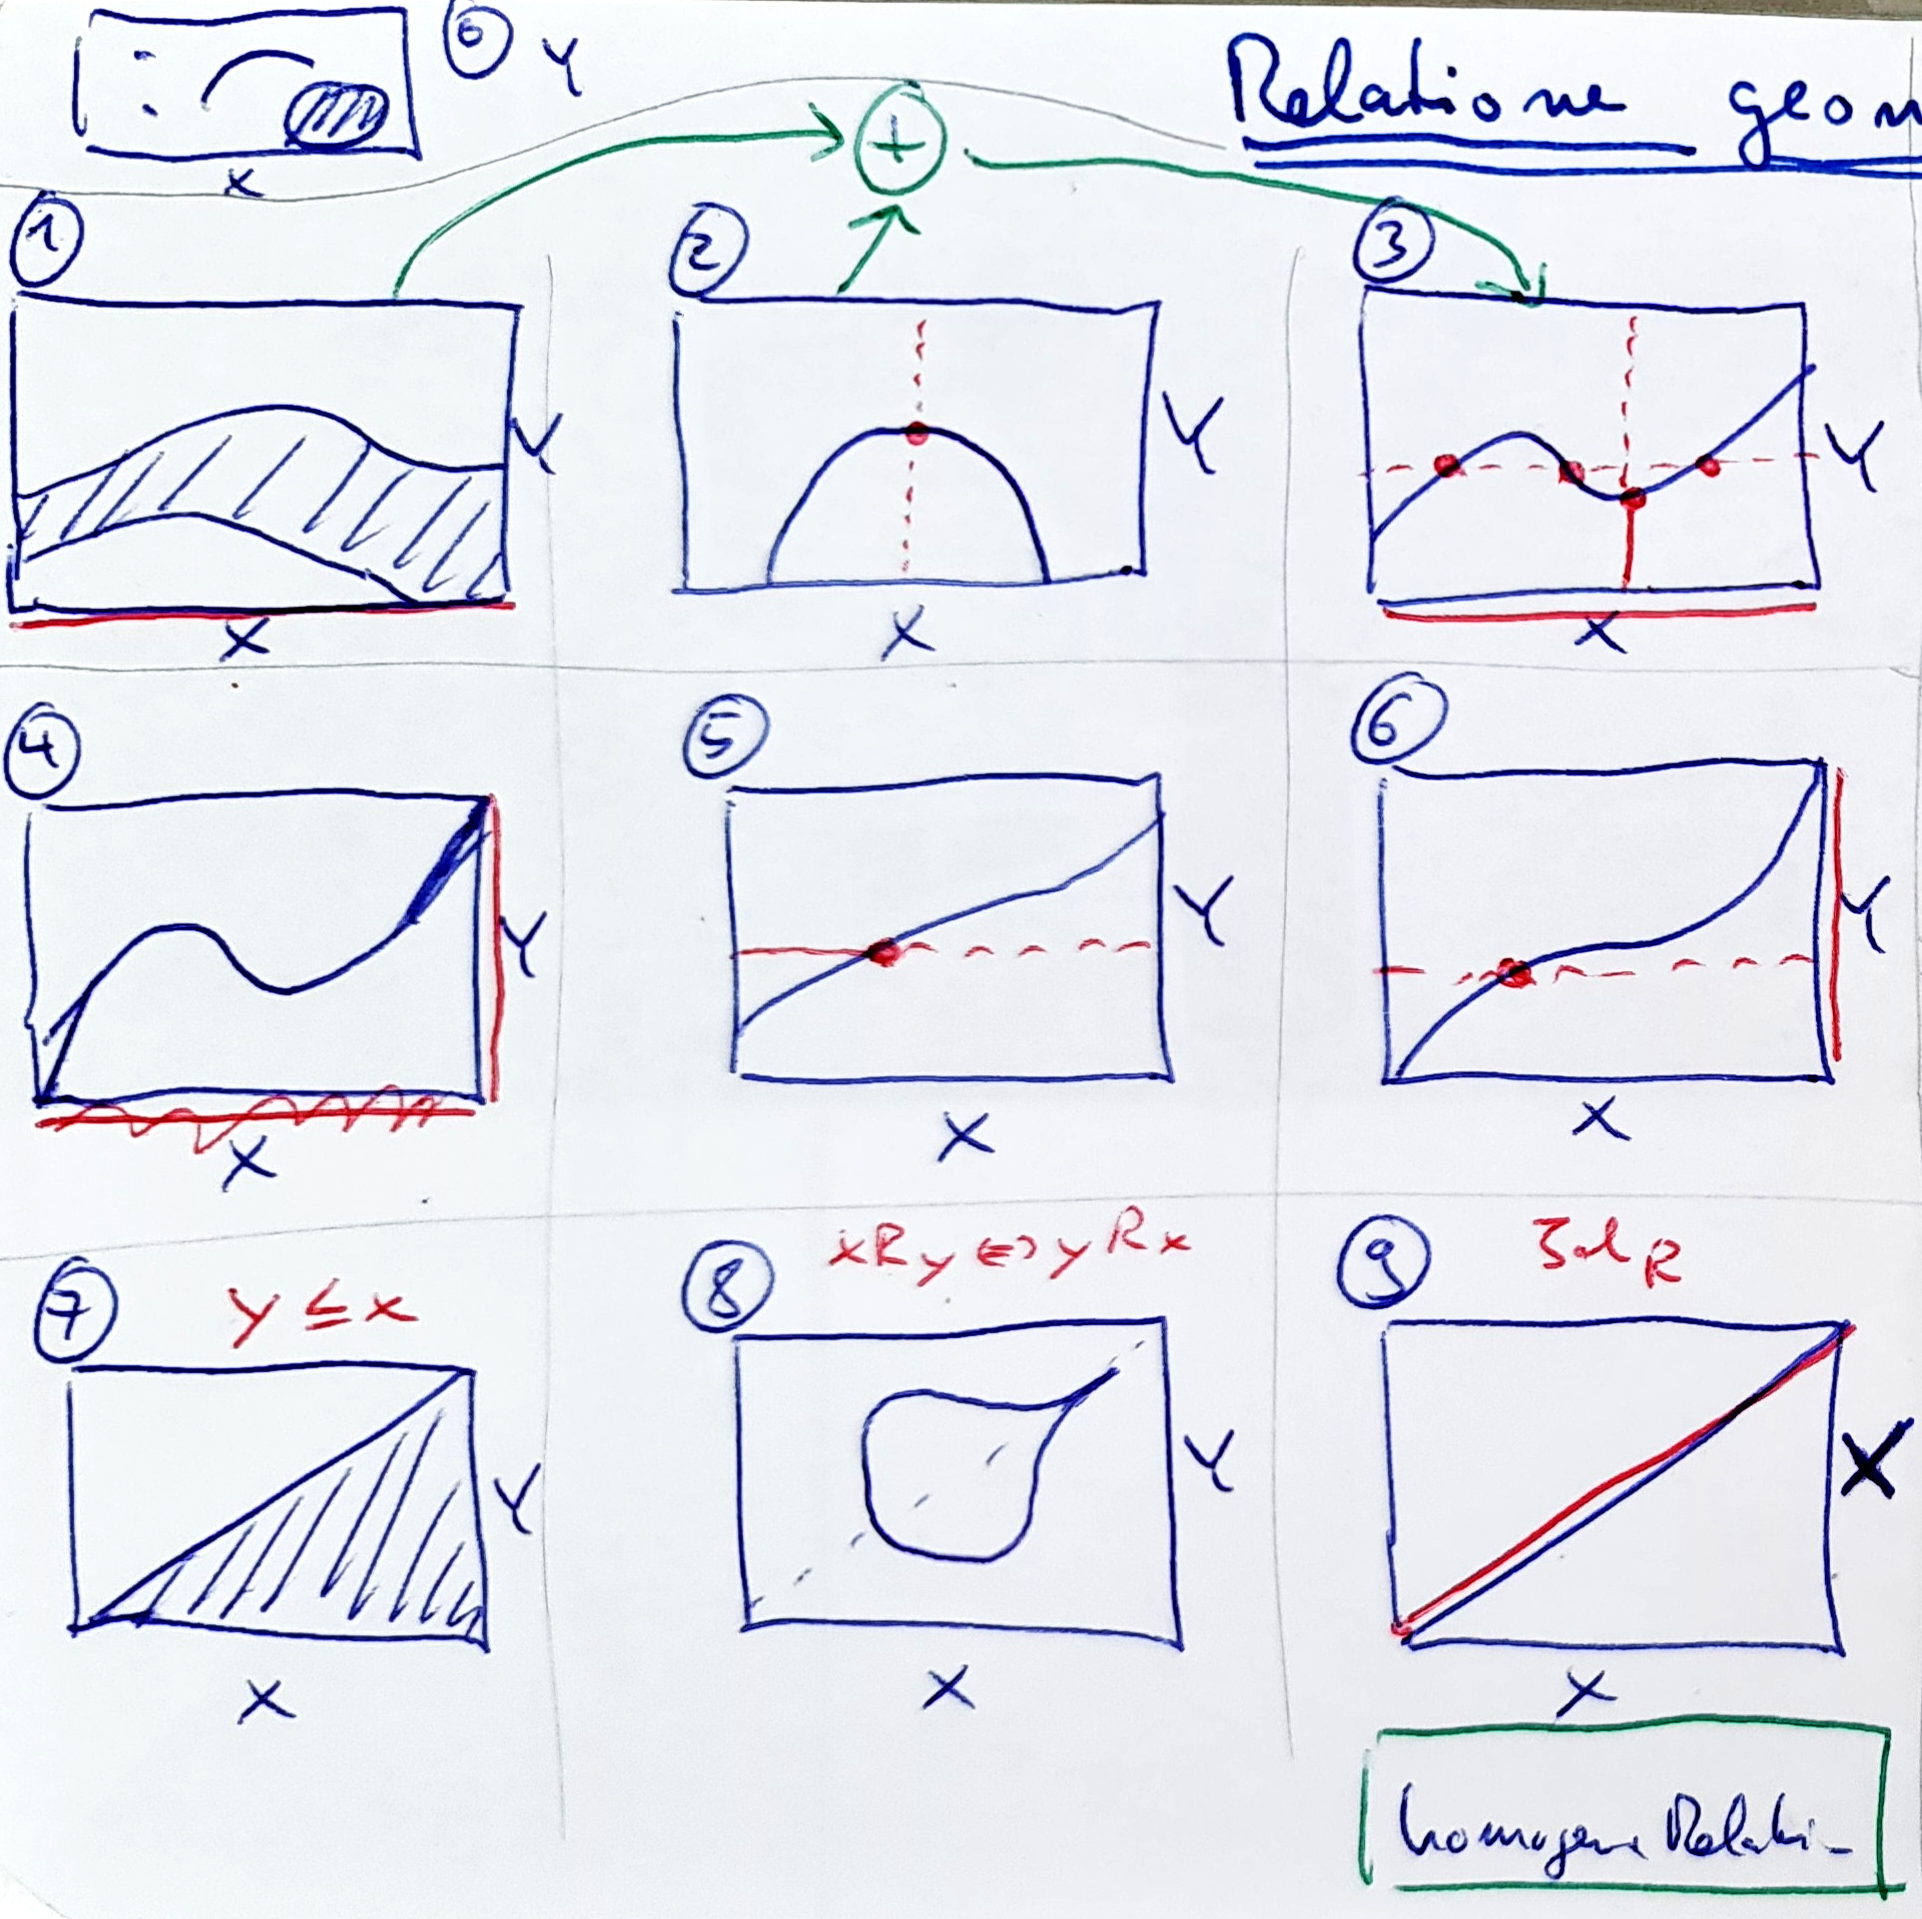
\includegraphics{v3.0.2.0.2 Relationen und Funktionen - Geometrisches Bild Grafik Links.png}
\end{figure}

\textbf{(5)} Die Relation ist links-vollständig, rechts-eindeutig und links-eindeutig. Eine injektive Funktion. Jeder $X$-Wert kommt genau einmal vor.

\textbf{(6)} Die Relation ist links-vollständig, rechts-vollständig, rechts-eindeutig und links-eindeutig. Eine bijektive Funktion. $X$- und $Y$-Werte stehen in einer 1:1 Beziehung.

\textbf{(7)} Angenommen $X$ und $Y$ sind tatsächlich Teilmengen des $\R^2$. Dann ist die schraffierte Fläche inklusive der Diagonalen die Relation $\le$. Da Relationen Teilmengen des kartesischen Produktes sind können wir schreiben
\begin{equation}
   \le \subseteq X \times Y.
\end{equation}

\textbf{(8)} Eine Relation $R \colon X - Y$ heißt \textbf{homogen}, falls $X=Y$. Es ist also eine Relation zwischen den Elementen einer Menge. Eine Relation ist symmetrisch, genau dann wenn
\begin{equation}
   x_1Rx_2 \Leftrightarrow x_2Rx_1.
\end{equation}
Die Grafik ist dann spiegelsymmetrisch bezüglich der Diagonalen.

\textbf{(9)} Die \textbf{Identität} $\id_X$ ist die Relation definiert durch
\begin{equation}
   x_1\id_Xx_2 \colon \Leftrightarrow x_1 = x_2.
\end{equation}
Intuitiv könnten wir also sagen, $\id_X$ ist das gleiche wie "`$=$"'. Formal ist das aber nicht so. $\id_X$ ist ein mathematischen Objekt, während "`$=$"' ein Zeichen unserer Sprache ist, welches nicht ein mathematisches Objekt bezeichnet.
Wir können durchaus sagen, dass $\id_X$ das mathematische Zeichen "`$=$"' als Objekt in das mathematische Universum inkarniert.

\begin{figure}
   \centering
   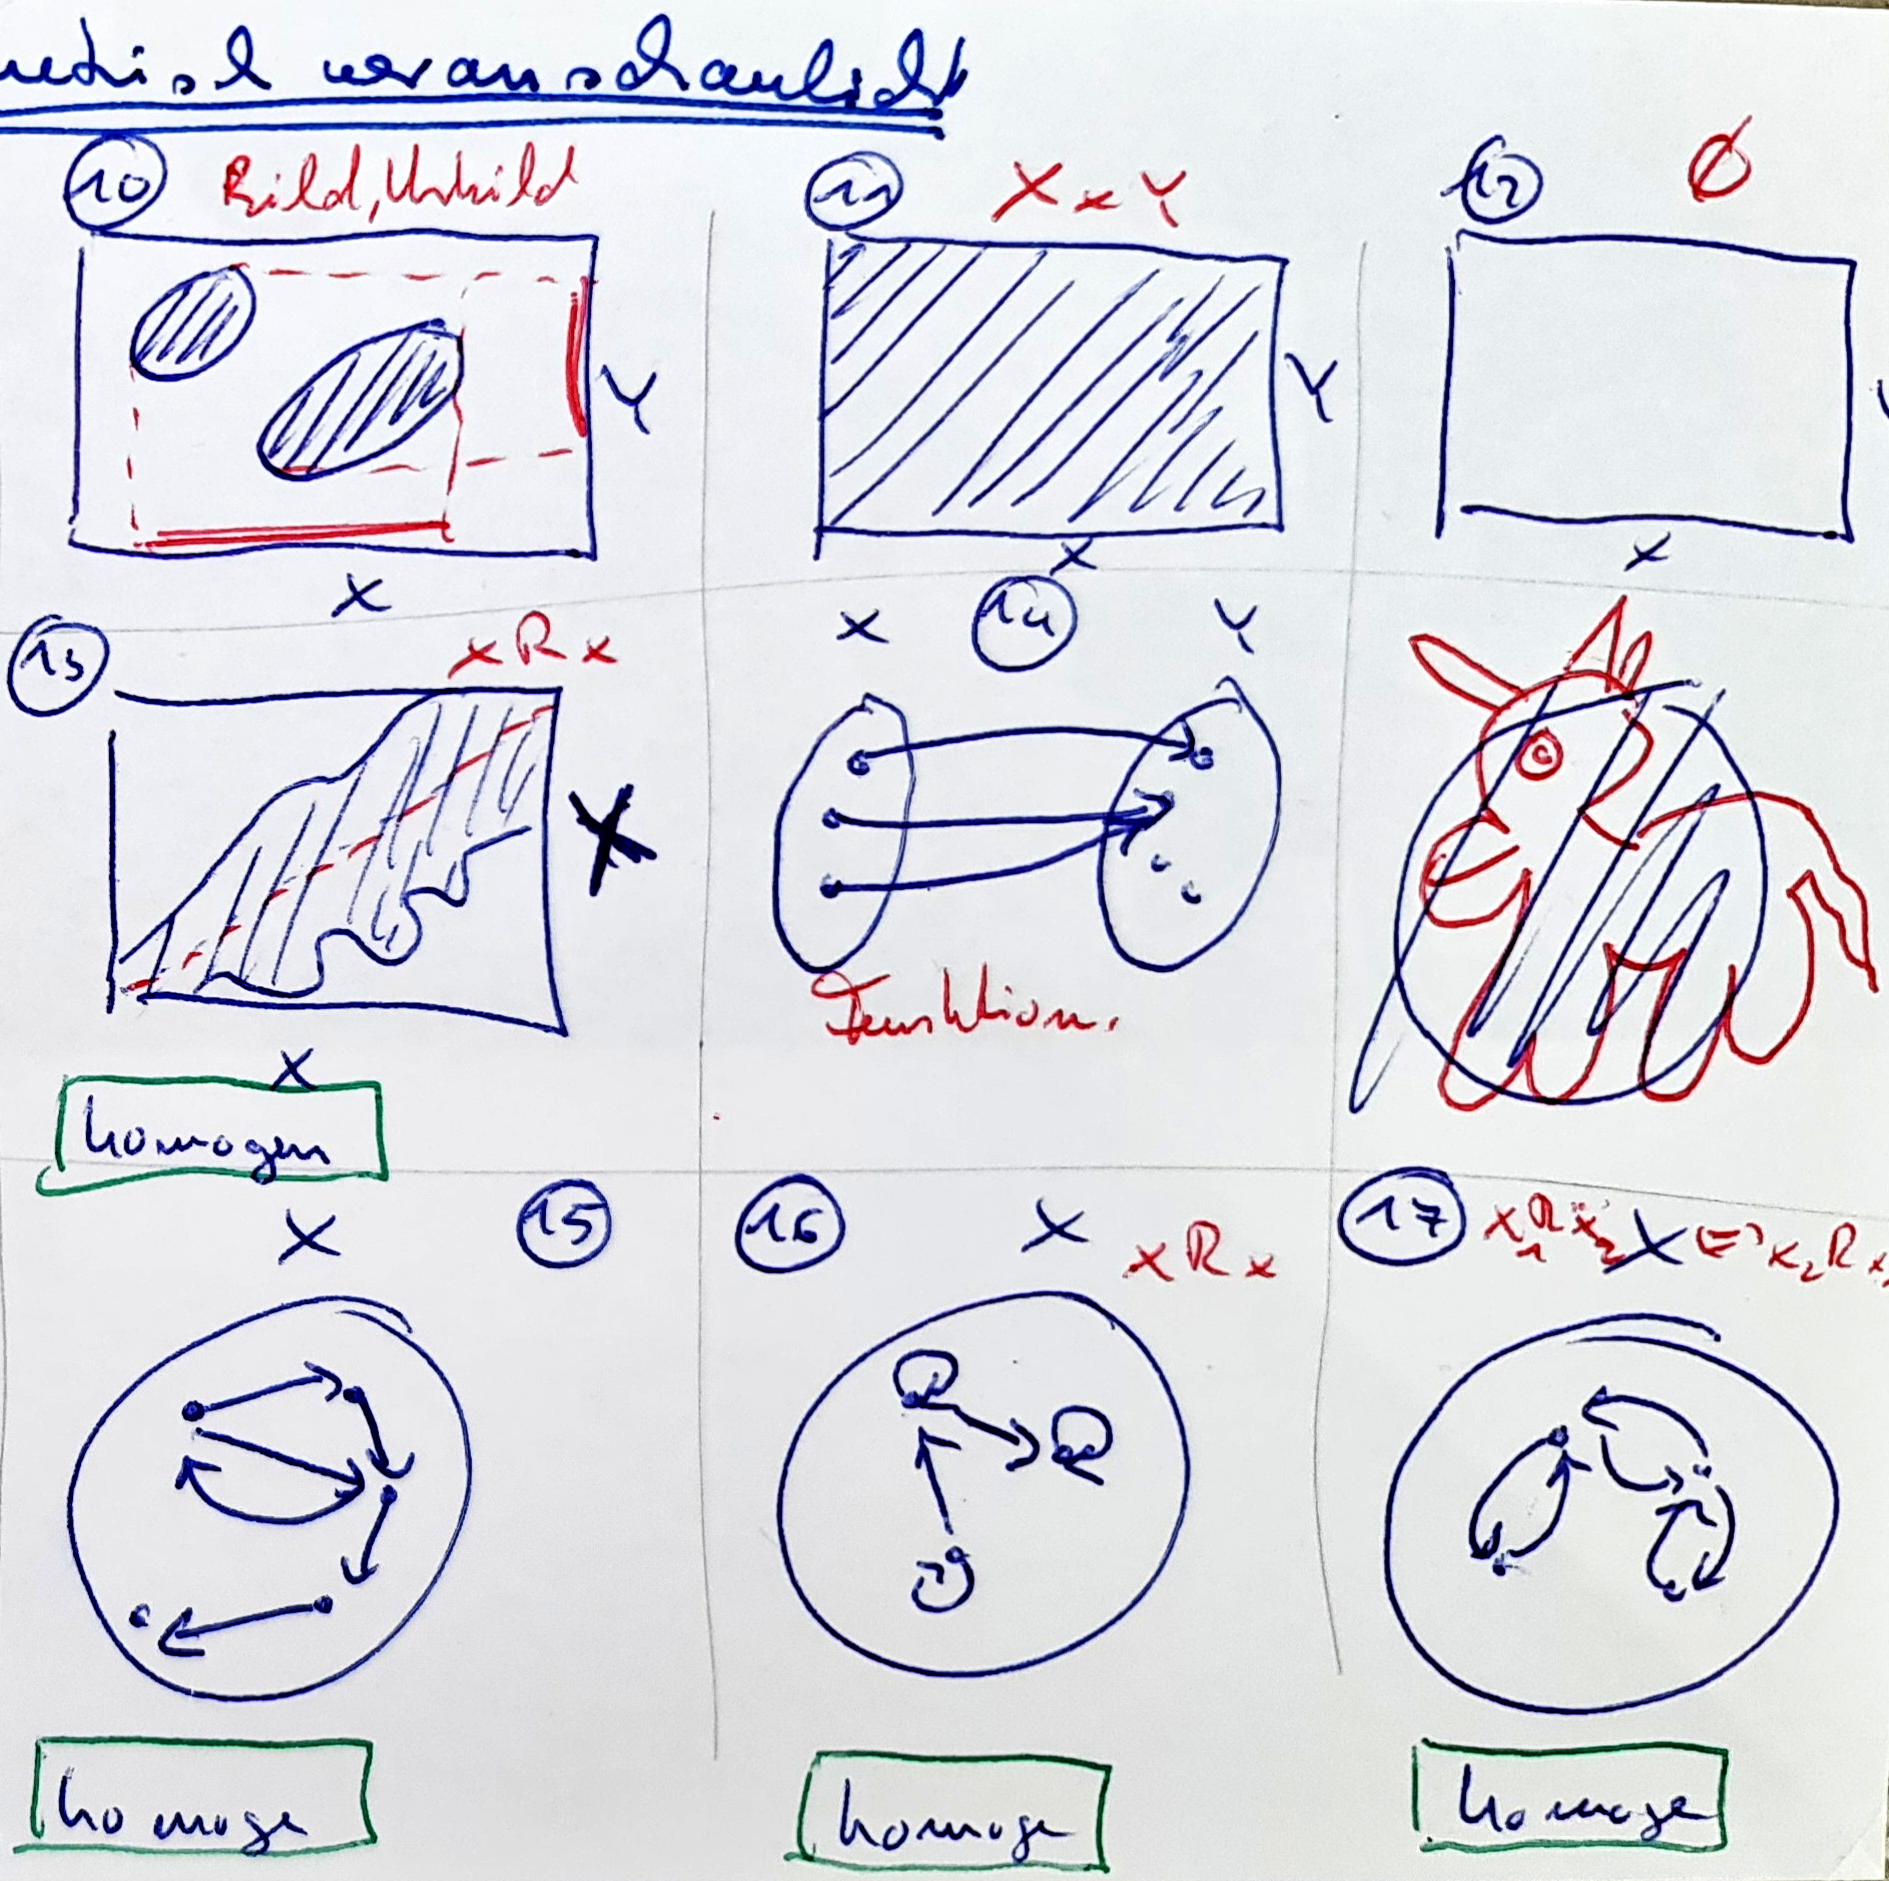
\includegraphics{v3.0.2.0.2 Relationen und Funktionen - Geometrisches Bild Grafik Rechts.png}
\end{figure}

\textbf{(10)} Sei $R$ eine Relation. Dann sind \textbf{Bild} und \textbf{Urbild} definiert als
\begin{align}
   \Bild R := \{ y \in Y &| \exists x \in X \colon xRy\}\\
   \Urbild R := \{ x \in X &| \exists y \in Y \colon xRy\}.
\end{align}

\textbf{(11)} Die \textbf{allgemeine Relation} ist einfach das kartesische Produkt $X \times Y$ selber.
Mit $R = X \times Y$ gilt somit gilt für alle $x \in X, y \in Y \colon xRy$.

\textbf{(12)} Die \textbf{leere Relation} oder \textbf{Null-Relation} ist die leere Menge (aufgefasst als Teilmenge von $X \times Y$).
Mit $R = \emptyset \subseteq X \times Y$ gilt somit gilt für kein $x \in X, y \in Y \colon xRy$.

\textbf{(13)} Eine homogene Relation $R \subseteq X \times X$ heisst \textbf{reflexiv}, wenn für alle $x\in X$ gilt $xRx$. In der Veranschaulichung heißt dies, dass die Diagonale in der Teilmenge liegt, die die Relation darstellt (die schraffierte Fläche).

%******************************************************************************************************
\subsection{Ellipsen und Pfeile zwischen den Elementen}
%******************************************************************************************************
\textbf{(14)} Die linke Ellipse entspricht $X$, die rechte $Y$. Die Elemente werde durch Punkte repräsentiert. Zwei solche Punkte $x \in X$ und $y \in Y$, für die $xRy$ werden durch einen Pfeil $x \mapsto y$ dargestellt. Ist die Relation links-vollständig, so hat jeder Punkt in $X$ einen Pfeil. Ist sie rechts-eindeutig, so hat jeder Punkt in $X$ nur einen Pfeil. Dargestellt ist eine Funktion, die beide Eigenschaften hat. Die dargestellte Funktion ist nicht injektiv, da zwei Pfeile auf das selbe Ziel-Objekt kommen. Sie ist nicht surjektiv, da es Punkte in $Y$ gibt, die keinen Pfeil abbekommen.
 
%******************************************************************************************************
\subsection{Gerichteten Graphen}
%******************************************************************************************************
Homogene Relationen könnten wir auch Endo-Relationen nennen: hier sind $X$ und $Y$ die selbe Menge.

\textbf{(15)} Homogene Relationen sind nichts anderes als gerichtete Graphen mit der Eingenschaft, dass es nur einen Pfeil von $x_1$ nach $x_2$ geben kann. Also \textbf{Endo-Relation = Nichtmulti-Digraph}. Ein wunderschönes Beispiel von zwei völlig verschiedenen Aspekten des selben Konzeptes.

\textbf{(16)} Bei einer homogenen reflexiven Relation (für alle $x\in X$ gilt $xRx$) haben dann alle Knoten einen Pfeil zu sich selbst (kleine Ohren).

\textbf{(17)} Bei einer homogenen symmetrischen Relation, $x_1Rx_2 \Leftrightarrow x_2Rx_1$, gibt es zu zwei Knoten entweder Pfeile in beiden Richtungen oder gar keinen. Damit ist das gleichbedeutend mit einem nicht-gerichteten Nichtmulti-Graph (idem wir aus jedem Hinundher-Paar eine einfache ungerichtete Kante machen).

\begin{backup}
%******************************************************************************************************
%                                                                                                     *
\section{TODO}
%                                                                                                     *
%******************************************************************************************************
Noch zu erledigen sind
\begin{itemize}
   \item leer
\end{itemize}
\end{backup}

\begin{backup}
    (Zur Zeit nicht benötigter Inhalt)
\end{backup}

%******************************************************************************************************
%                                                                                                     *
\begin{thebibliography}{9}
%                                                                                                     *
%******************************************************************************************************

   \bibitem[ArensBusamHettlichKarpfingerStachel2022]{Grundwissen}
      Tilo Arens, Rolf Busam, Frank Hettlich, Christian Karpfinger, Hellmuth Stachel, \emph{Grundwissen Mathematikstudium},
      Springer, 978-3-662-63312-0 (ISBN)
      
\end{thebibliography}

%******************************************************************************************************
%                                                                                                     *
\begin{large}
    \centerline{\textsc{Symbolverzeichnis}}
\end{large}
%                                                                                                     *
%******************************************************************************************************
\bigskip

\renewcommand*{\arraystretch}{1}

\begin{tabular}{ll}
    $X, Y, \cdots$          & Mengen\\
    $x, y, \cdots$             & Elemente\\
    $R$             & Eine Relation
   
\end{tabular}

\end{document}
